\section{Experimentación}

En esta sección mostraremos los resultados de las pruebas con los distintos preprocesados, modelos y parámetros.

\subsection{Primera derivada}

Para probar que, como hemos comentado antes, el aplicar la primera derivada sobre los datos nos puede ayudar a la hora de predecir, podemos comparar los resultados de entrenar con o sin derivar en la \textit{tabla\ \ref{tab:nopreprocessing-derivative-results}} y, efectivamente, obtenemos resultados algo mejores.

\begin{table}[!h]
    \centering
    \resizebox{\textwidth}{!}{\begin{tabular}{|c|ccccccc|ccccccc|}
        \hline
        & \multicolumn{7}{|c|}{Derivative} & \multicolumn{7}{c|}{No preprocessing} \\ \hline
        Model Name & Train score & Test score & f1score & f0.5score & f2score & ROC/AUC score & Balanced accuracy & Train score & Test score & f1score & f0.5score & f2score & ROC/AUC score & Balanced accuracy \\ \hline
        XGBoost & 82 & 82 & 0 & 0 & 0 & 50 & 50 & 82 & 82 & 0 & 0 & 0 & 50 & 50 \\
        Stochastic Gradient Descent & 18 & 18 & 30.508 & 21.531 & 52.326 & 50 & 50 & 18 & 18 & 30.508 & 21.531 & 52.326 & 50 & 50 \\
        Random Forest & 99.926 & 87.778 & 49.541 & 69.948 & 38.352 & 66.531 & 66.531 & 99.556 & 84.889 & 52.778 & 57.057 & 49.096 & 70.069 & 70.069 \\
        Quadratic Discriminant Analysis & 100 & 82 & 0 & 0 & 0 & 50 & 50 & 100 & 82 & 0 & 0 & 0 & 50 & 50 \\
        Multi-Layer Perceptron & 83.259 & 80.667 & 8.421 & 14.599 & 5.917 & 51.114 & 51.114 & 82 & 82 & 0 & 0 & 0 & 50 & 50 \\
        Linear Discriminant Analysis & 85.333 & 78.222 & 20.968 & 25.692 & 17.711 & 53.96 & 53.96 & 84.889 & 78 & 22.047 & 26.415 & 18.919 & 54.306 & 54.306 \\
        LightGBM & 81.852 & 72 & 47.934 & 40 & 59.794 & 71.846 & 71.846 & 75.778 & 64 & 37.692 & 30.74 & 48.708 & 62.632 & 62.632 \\
        K-Neighbors & 100 & 86.889 & 56.296 & 63.973 & 50.265 & 71.289 & 71.289 & 100 & 91.778 & 74.83 & 79.71 & 70.513 & 82.46 & 82.46 \\
        Hist Gradient Boosting & 78.444 & 70.444 & 44.813 & 37.448 & 55.785 & 68.97 & 68.97 & 72.815 & 63.556 & 33.871 & 28.037 & 42.77 & 58.988 & 58.988 \\
        Extra Trees & 99.63 & 90.444 & 69.504 & 76.324 & 63.802 & 78.756 & 78.756 & 94.667 & 81.111 & 56.853 & 51.376 & 63.636 & 76.438 & 76.438 \\
        Decision Tree & 56.963 & 58.889 & 41.27 & 31.957 & 58.244 & 67.224 & 67.224 & 82 & 82 & 0 & 0 & 0 & 50 & 50 \\ \hline
        & & & & & & 61.79 & 61.79 & & & & & & 59.53572727 & 59.53572727 \\ \hline
        \end{tabular}}
    \caption{Comparación de los resultados de entrenar utilizando la derivada y sin preprocesar. Fuente propia.}\ \label{tab:nopreprocessing-derivative-results}
\end{table}

\subsection{Transformada}

Podemos ver los resultados de entrenar utilizando la transformada sobre los datos derivados en la \textit{tabla\ \ref{tab:derivative-transformed-results}}, vemos que los resultados son algo peores, así que continuaremos las pruebas sin utilizar la transformada.

\begin{table}[!h]
    \centering
    \resizebox{\textwidth}{!}{\begin{tabular}{|c|ccccccc|ccccccc|}
        \hline
            & \multicolumn{7}{|c|}{Transformer and derivative} & \multicolumn{7}{c|}{Derivative} \\ \hline
            Model Name & Train score & Test score & f1score & f0.5score & f2score & ROC/AUC score & Balanced accuracy & Train score & Test score & f1score & f0.5score & f2score & ROC/AUC score & Balanced accuracy \\ \hline
            XGBoost & 82 & 82 & 0 & 0 & 0 & 50 & 50 & 82 & 82 & 0 & 0 & 0 & 50 & 50 \\
            Stochastic Gradient Descent & 18 & 18 & 30.508 & 21.531 & 52.326 & 50 & 50 & 18 & 18 & 30.508 & 21.531 & 52.326 & 50 & 50 \\
            Random Forest & 99.926 & 87.778 & 49.541 & 69.948 & 38.352 & 66.531 & 66.531 & 99.926 & 87.778 & 49.541 & 69.948 & 38.352 & 66.531 & 66.531 \\
            Quadratic Discriminant Analysis & 100 & 83.333 & 19.355 & 34.884 & 13.393 & 55.149 & 55.149 & 100 & 82 & 0 & 0 & 0 & 50 & 50 \\
            Multi-Layer Perceptron & 82 & 82 & 0 & 0 & 0 & 50 & 50 & 83.259 & 80.667 & 8.421 & 14.599 & 5.917 & 51.114 & 51.114 \\
            Linear Discriminant Analysis & 85.185 & 76.667 & 18.605 & 21.978 & 16.129 & 52.529 & 52.529 & 85.333 & 78.222 & 20.968 & 25.692 & 17.711 & 53.96 & 53.96 \\
            LightGBM & 81.852 & 72 & 47.934 & 40 & 59.794 & 71.846 & 71.846 & 81.852 & 72 & 47.934 & 40 & 59.794 & 71.846 & 71.846 \\
            K-Neighbors & 100 & 80.222 & 25.21 & 32.189 & 20.718 & 56.143 & 56.143 & 100 & 86.889 & 56.296 & 63.973 & 50.265 & 71.289 & 71.289 \\
            Hist Gradient Boosting & 78.444 & 70.444 & 44.813 & 37.448 & 55.785 & 68.97 & 68.97 & 78.444 & 70.444 & 44.813 & 37.448 & 55.785 & 68.97 & 68.97 \\
            Extra Trees & 99.63 & 90 & 68.966 & 74.184 & 64.433 & 78.967 & 78.967 & 99.63 & 90.444 & 69.504 & 76.324 & 63.802 & 78.756 & 78.756 \\
            Decision Tree & 56.963 & 58.889 & 41.27 & 31.957 & 58.244 & 67.224 & 67.224 & 56.963 & 58.889 & 41.27 & 31.957 & 58.244 & 67.224 & 67.224 \\ \hline
            & & & & & & 60.669 & 60.669 & & & & & & 61.79 & 61.79 \\ \hline
        \end{tabular}}
    \caption{Comparación de los resultados de entrenar transformando y derivando los datos; frente a solo derivando. Fuente propia.}\ \label{tab:derivative-transformed-results}
\end{table}

\subsection{Estandarización}

Al aplicar la estandarización de los datos después de derivarlos obtenemos los resultados de la \textit{tabla\ \ref{tab:derivative-standarization-results}}, los cuales son mejores que los anteriores.


\begin{table}[!h]
    \resizebox{\textwidth}{!}{\begin{tabular}{|c|ccccccc|ccccccc|}
        \hline
        & \multicolumn{7}{c|}{Derivative + Scaler} & \multicolumn{7}{c|}{Derivative} \\ \hline
        Model Name & Train score & Test score & f1score & f0.5score & f2score & ROC/AUC score & Balanced accuracy & Train score & Test score & f1score & f0.5score & f2score & ROC/AUC score & Balanced accuracy \\ \hline
        XGBoost & 82 & 82 & 0 & 0 & 0 & 50 & 50 & 82 & 82 & 0 & 0 & 0 & 50 & 50 \\
        Stochastic Gradient Descent & 64.815 & 56.444 & 24.615 & 20.075 & 31.809 & 49.834 & 49.834 & 18 & 18 & 30.508 & 21.531 & 52.326 & 50 & 50 \\
        Random Forest & 99.926 & 87.778 & 49.541 & 69.948 & 38.352 & 66.531 & 66.531 & 99.926 & 87.778 & 49.541 & 69.948 & 38.352 & 66.531 & 66.531 \\
        Quadratic Discriminant Analysis & 96.148 & 83.111 & 54.217 & 53.444 & 55.012 & 72.358 & 72.358 & 100 & 82 & 0 & 0 & 0 & 50 & 50 \\
        Multi-Layer Perceptron & 90.815 & 84 & 32.075 & 46.961 & 24.355 & 59.41 & 59.41 & 83.259 & 80.667 & 8.421 & 14.599 & 5.917 & 51.114 & 51.114 \\
        Linear Discriminant Analysis & 85.333 & 78.222 & 20.968 & 25.692 & 17.711 & 53.96 & 53.96 & 85.333 & 78.222 & 20.968 & 25.692 & 17.711 & 53.96 & 53.96 \\
        LightGBM & 82.222 & 72.222 & 48.133 & 40.222 & 59.917 & 71.981 & 71.981 & 81.852 & 72 & 47.934 & 40 & 59.794 & 71.846 & 71.846 \\
        K-Neighbors & 100 & 86.889 & 55.639 & 64.014 & 49.202 & 70.807 & 70.807 & 100 & 86.889 & 56.296 & 63.973 & 50.265 & 71.289 & 71.289 \\
        Hist Gradient Boosting & 78.444 & 70.444 & 44.813 & 37.448 & 55.785 & 68.97 & 68.97 & 78.444 & 70.444 & 44.813 & 37.448 & 55.785 & 68.97 & 68.97 \\
        Extra Trees & 99.63 & 90.444 & 69.504 & 76.324 & 63.802 & 78.756 & 78.756 & 99.63 & 90.444 & 69.504 & 76.324 & 63.802 & 78.756 & 78.756 \\
        Decision Tree & 56.963 & 58.889 & 41.27 & 31.957 & 58.244 & 67.224 & 67.224 & 56.963 & 58.889 & 41.27 & 31.957 & 58.244 & 67.224 & 67.224 \\ \hline
        & & & & & & 64.53009091 & 64.53009091 & & & & & & 61.79 & 61.79 \\ \hline
        \end{tabular}}
    \caption{Comparación de los resultados de entrenar derivando y estandarizando los datos; frente a solo derivando. Fuente propia.}\ \label{tab:derivative-standarization-results}
\end{table}


\subsection{Aumento y disminución de dimensionalidad}

Aun siendo un paso generalmente recomendado, el aumento y disminución de dimensionalidad nos ha dado los resultados de la \textit{tabla\ \ref{tab:derivative-standarization-dimensionality-results}}, los cuales son algo peores que los anteriores, por lo cual, no aplicaremos estas técnicas en los siguientes pasos.

\begin{table}[!h]
    \resizebox{\textwidth}{!}{\begin{tabular}{|c|ccccccc|ccccccc|}
        \hline
            & \multicolumn{7}{c|}{Derivative + Scaler + Polynomial Features + PCA} & \multicolumn{7}{c|}{Derivative + Scaler} \\ \hline
            Model Name & Train score & Test score & f1score & f0.5score & f2score & ROC/AUC score & Balanced accuracy & Train score & Test score & f1score & f0.5score & f2score & ROC/AUC score & Balanced accuracy \\ \hline
            XGBoost & 82 & 82 & 0 & 0 & 0 & 50 & 50 & 82 & 82 & 0 & 0 & 0 & 50 & 50 \\
            Stochastic Gradient Descent & 53.333 & 50.444 & 28.754 & 22.299 & 40.468 & 52.439 & 52.439 & 64.815 & 56.444 & 24.615 & 20.075 & 31.809 & 49.834 & 49.834 \\
            Random Forest & 99.926 & 85.778 & 38.462 & 57.803 & 28.818 & 61.939 & 61.939 & 99.926 & 87.778 & 49.541 & 69.948 & 38.352 & 66.531 & 66.531 \\
            Quadratic Discriminant Analysis & 80.889 & 80 & 40 & 42.017 & 38.168 & 63.234 & 63.234 & 96.148 & 83.111 & 54.217 & 53.444 & 55.012 & 72.358 & 72.358 \\
            Multi-Layer Perceptron & 87.778 & 81.778 & 19.608 & 30.303 & 14.493 & 54.682 & 54.682 & 90.815 & 84 & 32.075 & 46.961 & 24.355 & 59.41 & 59.41 \\
            Linear Discriminant Analysis & 82.741 & 81.111 & 6.593 & 12.397 & 4.491 & 50.903 & 50.903 & 85.333 & 78.222 & 20.968 & 25.692 & 17.711 & 53.96 & 53.96 \\
            LightGBM & 77.037 & 68.444 & 38.261 & 32.496 & 46.512 & 62.933 & 62.933 & 82.222 & 72.222 & 48.133 & 40.222 & 59.917 & 71.981 & 71.981 \\
            K-Neighbors & 100 & 83.778 & 42.52 & 50.943 & 36.486 & 64.092 & 64.092 & 100 & 86.889 & 55.639 & 64.014 & 49.202 & 70.807 & 70.807 \\
            Hist Gradient Boosting & 75.63 & 66 & 37.037 & 30.864 & 46.296 & 61.924 & 61.924 & 78.444 & 70.444 & 44.813 & 37.448 & 55.785 & 68.97 & 68.97 \\
            Extra Trees & 96.222 & 82.222 & 51.22 & 50.847 & 51.597 & 70.37 & 70.37 & 99.63 & 90.444 & 69.504 & 76.324 & 63.802 & 78.756 & 78.756 \\
            Decision Tree & 71.852 & 68.889 & 27.835 & 25.328 & 30.892 & 55.014 & 55.014 & 56.963 & 58.889 & 41.27 & 31.957 & 58.244 & 67.224 & 67.224 \\ \hline
            & & & & & & 58.86636364 & 58.86636364 & & & & & & 64.53009091 & 64.53009091 \\ \hline
        \end{tabular}} 
    \caption{Comparación de los resultados de entrenar derivando, estandarizando y ajustando la dimensionalidad de los datos; frente a solo derivando y estandarizando. Fuente propia.}\ \label{tab:derivative-standarization-dimensionality-results}
\end{table}


\subsection{Selección de modelos y \textit{hyperparameter tuning}}\ \label{sec:entrenamiento}

Una vez encontrada una combinación de pasos de preprocesado que nos mejora los resultados, podemos pasar al siguiente paso de selección de los modelos. Habiendo entrenado ya los modelos, vemos que algunos hacen \textit{overfitting}. El \textit{overfitting} ocurre cuando un modelo se ajusta demasiado a los datos con los que ha entrenado y no generaliza bien, es decir que predice mejor los datos con los que ha entrenado que datos nuevos. Donde lo podemos ver más claramente es en \textit{KNeighbors}, vemos en la \textit{figura\ \ref{fig:lc-knn}} que, para cualquier cantidad de datos con los que entrenemos el modelo, siempre predecirá bien con los que ha entrenado y no tanto con los demás. Nuestro objetivo es intentar que ambos valores no sean tan dispares y que sean lo más altos posibles, para ello haremos \textit{hyperparameter tuning}.

\begin{figure}[!h]
    \centering
    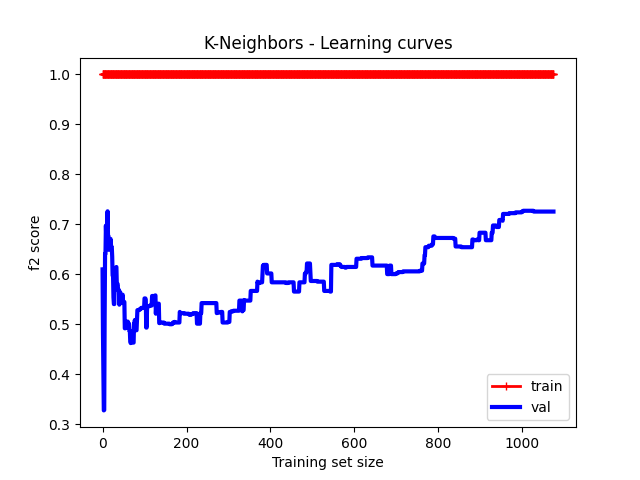
\includegraphics[width=0.7\linewidth]{media/images/learing-curves-knn.png}
    \caption{Gráfico de la curva de aprendizaje del modelo \textit{K-Neighbors} entrenándolo y probándolo sobre los datos de entreno únicamente. Fuente propia}\ \label{fig:lc-knn}
\end{figure}

Para evitar el \textit{overfitting}, uno de los posibles remedios es utilizar \textit{hyperparameter tuning}. El \textit{hyperparameter tuning} tiene como objetivo encontrar un conjunto de parámetros que maximice el rendimiento del modelo sobre los datos de prueba. En nuestro caso, como los datos están desbalanceados, podemos utilizar como función de rendimiento el \textit{balanced accuracy}. Como cada modelo es distinto, debemos encontrar los parámetros adecuados para cada uno. 

Para ahorrarnos tiempo podemos utilizar solamente los mejores modelos, como hemos visto en los resultados de la \textit{tabla\ \ref{tab:derivative-standarization-dimensionality-results}}, hay modelos que tienen mejores resultados que otros. Así que escogeremos los cuatro con mejor \textit{balanced accuracy}, es decir: \textit{Extra Trees, Quadratic Discriminant Analysis, LightGBM y K-Neighbors}.

Realizaremos el \textit{hyperparameter tuning} en dos pasos, primeramente utilizaremos \textit{Random Search} y después \textit{Grid Search}, ya implementados en \textit{sklearn}.
Ambos métodos utilizan \textit{cross-validation}, una técnica para evitar el \textit{overfitting} que consiste en la división de los datos de entreno en partes iguales.
Una vez dividido en \textit{N} partes, se entrena el modelo sobre todas las partes excepto una, la cual se utiliza para evaluar el modelo entrenado. Entonces, se repite el 
proceso cambiando de partición. De esta forma, haciendo la media obtenemos el resultado de entrenar el modelo repetidas ocasiones con los mismos parámetros, pero con datos 
distintos. Una vez hemos obtenido el mejor de los modelos que hemos entrenado, según la función de rendimiento, probamos el modelo resultante sobre los datos de prueba.
Podemos ver este proceso más gráficamente en la \textit{imagen\ \ref{fig:cross-validation}}.

\begin{figure}[!h]
    \centering
    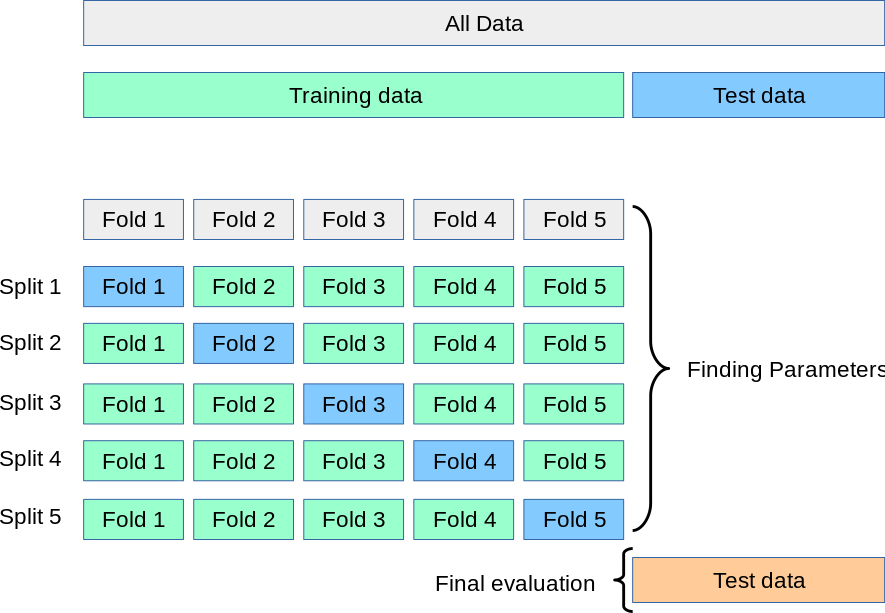
\includegraphics[width=0.7\linewidth]{media/images/cross-validation.png}
    \caption{\textit{Cross-validation} explicado gráficamente. Fuente:\ \cite{31Crossv20:online}}\ \label{fig:cross-validation}
\end{figure}


El \textit{random search} consiste en la búsqueda de estos parámetros habiendo definido un rango de posibilidades. Es decir, para cada parámetro que le queramos
pasar al modelo definiremos un rango de valores que puede tener, entonces el \textit{random search} entrena el modelo repetidas veces con una permutación aleatoria de sus 
parámetros y se guarda los resultados. Podemos ver un ejemplo en el \textit{código\ \ref{code:random-search-example}}.
Podemos ir probando diferentes parámetros y rangos hasta que estemos satisfechos con el resultado.


Una vez estemos contentos con los resultados, los refinaremos utilizando \textit{grid search}. A diferencia del \textit{random search}, el \textit{grid search} prueba todas
las posibles combinaciones que le pasemos como parámetro y, consecuentemente, es mucho más lento. Por ello, utilizaremos el \textit{grid search} con los mejores parámetros que
encontremos del paso anterior, los cuales son potencialmente los mejores. Una vez definido un rango de parámetros para los modelos seleccionados, obtenemos los resultados
de la \textit{tabla\ \ref{tab:hyperparameter-tuning-results}}. Podemos ver que hemos obtenido, en general, peores resultados (salvo con \textit{K-Neighbors}), por lo tanto
deberíamos ajustar el rango de parámetros que les pasamos a los modelos y volver a entrenarlos hasta que estemos satisfechos con el resultado. En nuestro caso no lo haremos
y pasaremos a la segunda iteración del proyecto para probar nuevas cosas en pasos anteriores.

\begin{table}
    \resizebox{\textwidth}{!}{\begin{tabular}{|c|ccccccc|}
            \hline
            Model name & Train score & Accuracy & f1 score & f0.5 score & f2 score & ROC/AUC score & Balanced accuracy \\ \hline
            RS - knn & 100 & 90.274 & 85.897 & 87.927 & 83.96 & 90.274 & 90.274 \\
            GS - knn & 100 & 90.274 & 85.897 & 87.927 & 83.96 & 90.274 & 90.274 \\
            RS - qda & 97.491 & 72.358 & 54.217 & 53.444 & 55.012 & 72.358 & 72.358 \\
            GS - qda & 97.491 & 72.358 & 54.217 & 53.444 & 55.012 & 72.358 & 72.358 \\
            RS - lgbm & 86.013 & 71.018 & 47.257 & 39.716 & 58.333 & 71.018 & 71.018 \\
            GS - et & 82.957 & 66.17 & 43.077 & 39.106 & 47.945 & 66.17 & 66.17 \\
            GS - lgbm & 84.628 & 70.626 & 46.215 & 38.108 & 58.704 & 70.626 & 70.626 \\
            RS - et & 69.492 & 65.854 & 40.909 & 33.21 & 53.254 & 65.854 & 65.854 \\\hline
            \end{tabular}
    }
    \caption{Resultados del primer entrenamiento con hyperparameter tuning. Fuente propia.}\ \label{tab:hyperparameter-tuning-results}
\end{table}

\subsection{Balanceo de datos}\ \label{sec:i2-balance}

\subsubsection{\textit{Undersampling}}

Al probar los algoritmos mencionados anteriormente, obtenemos los resultados de la \textit{tabla\ \ref{tab:undersampling-methods}}. Podemos ver que, en general, tanto los diferentes \textit{Near Miss} como el \textit{RUS}, obtienen resultados bastante peores que los otros métodos. En cuanto a los otros tres algoritmos restantes, el \textit{ENN (ALL)} es el que mejores resultados tiene, así que continuaremos utilizándolo.

Podemos ver en la \textit{figura\ \ref{fig:balance-enn}} la comparación del balance de la clase objetivo antes y después de utilizar el método \textit{ENN (ALL)}. 

\begin{table}[!ht]
    \resizebox{\textwidth}{!}{\begin{tabular}{|c|ccc|} \hline
        & Avg. f0.5 Score & Avg. f2 Score & Avg. Balanced Accuracy \\ \hline
        Random Under Sampler & 26.077 & 41.954 & 63.656 \\
        Near Miss (v1) & 28.814 & 53.698 & 62.754 \\
        Near Miss (v2) & 27.377 & 53.592 & 61.315 \\
        Near Miss (v3) & 24.800 & 39.654 & 61.999 \\
        Edited Nearest Neighbors (ALL) & 40.625 & 46.600 & 66.523 \\
        Edited Nearest Neighbors (MODE) & 41.130 & 42.018 & 64.575 \\
        Tomek Links & 42.415 & 42.610 & 65.236 \\ \hline
        \end{tabular}}
    \caption{Resultado de entrenar los modelos básicos sobre el \textit{dataset} reducido con los diferentes métodos. Fuente: propia.}\ \label{tab:undersampling-methods}
\end{table}

\begin{figure}[!ht]
    \centering
    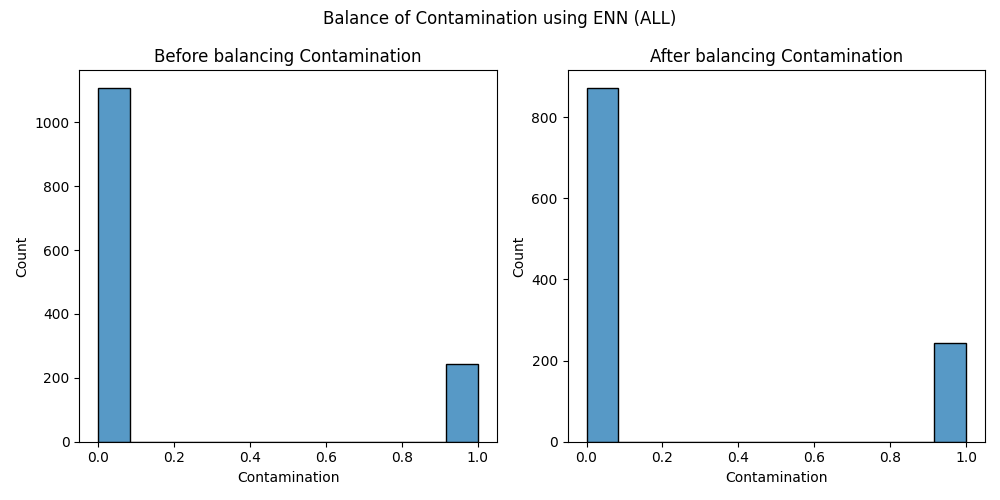
\includegraphics[width=0.8\linewidth]{media/images/balance.png}
    \caption{Comparación del balance de la clase objetivo antes y después de utilizar el método de \textit{undersampling ENN (ALL)}. Fuente propia.}\ \label{fig:balance-enn}
\end{figure}

\clearpage

\subsubsection{\textit{Oversampling}}

Antes de comentar los sintetizadores que probaremos, definiremos el método con los que los evaluaremos los datos generados. Utilizaremos una función de la propia librería \textit{sdv} que evalúa la similitud estadística de los datos generados con los datos reales y nos genera un \textit{quality report}.

Una vez hemos entrenado los sintetizadores, evaluamos su similitud con los datos reales y obtenemos los resultados de la \textit{tabla\ \ref{tab:oversampling-quality-report}}, en los cuales podemos ver un claro `ganador'.

\begin{table}[!ht]
    \centering
    \resizebox{0.8\linewidth}{!}{\begin{tabular}{|c|ccc|} \hline
        Synthesizer & Column Shapes & Column Pair Trends & Overall Quality \\ \hline
        Gaussian Copula Synthesizer & 94.75 & 99.83 & 97.29 \\
        TVAE Synthesizer & 84.37 & 74.97 & 79.64 \\ \hline
        CTGAN Synthesizer & - & - & - \\ 
        CopulaGAN Synthesizer & - & - & - \\ \hline
    \end{tabular}}
    \caption{Resultados del \textit{quality report} de los datos generados con los sintetizadores. Fuente propia}\ \label{tab:oversampling-quality-report}
\end{table}

Ahora que tenemos el sintetizador que mejores resultados nos da, lo aplicamos sobre la clase minoritaria y generamos datos sintéticos. Una vez generados, entrenamos los modelos básicos y obtenemos los resultados de la \textit{tabla\ \ref{tab:balanced-basic-training}}. Podemos ver que, en general, son peores que sin utilizar ningún sintetizador, por lo tanto, no utilizaremos \textit{oversampling} en los siguientes pasos.


\begin{table}[!ht]
    \centering
    \resizebox{\textwidth}{!}{\begin{tabular}{|c|cc|ccc|}\hline
        Model Name & Train score & Test score & f0.5score & f2score & Balanced accuracy \\ \hline
        XGBoost & 89.908 & 78.889 & 30.189 & 21.622 & 55.812 \\
        Stochastic Gradient Descent & 79.53 & 69.333 & 23.952 & 27.972 & 53.839 \\
        Random Forest & 97.42 & 82.444 & 48.961 & 42.526 & 66.17 \\
        Quadratic Discriminant Analysis & 93.005 & 82.667 & 28 & 10.448 & 53.779 \\
        Multi-Layer Perceptron & 94.209 & 80.889 & 44.818 & 40.712 & 64.74 \\
        Linear Discriminant Analysis & 87.041 & 76.889 & 24.561 & 18.667 & 53.628 \\
        LightGBM & 90.195 & 77.111 & 21.401 & 14.946 & 52.319 \\
        K-Neighbors & 100 & 85.778 & 60.533 & 61.425 & 76.393 \\
        Hist Gradient Boosting & 86.812 & 77.333 & 22.989 & 16.26 & 52.936 \\
        Extra Trees & 90.998 & 80 & 35.316 & 25.606 & 57.934 \\
        Decision Tree & 83.658 & 80.222 & 16.34 & 7.31 & 51.325 \\ \hline
        Average & & & 32.460 & 26.135 & 58.079 \\ \hline
        \end{tabular}}
    \caption{Resultados de entrenar los modelos básicos habiendo balanceado el \textit{dataset}. Fuente propia.}\ \label{tab:balanced-basic-training}
\end{table}

\clearpage
\subsection{Nuevos modelos}

Hay dos tipos de modelos más complejos que no hemos probado que pueden darnos mejores resultados, estos son \textit{Voting Classifier} y \textit{Bagging Classifier}. El primero, \textit{Voting Classifier}, entrena los modelos que lo componen sobre el \textit{dataset} y, a la hora de predecir, se basa en las predicciones de estos modelos. Es decir, realiza una votación y la clase que más se vote es la que sale como predicción como podemos ver en la \textit{figura\ \ref{fig:voting-classifiers}}. Hay dos tipos de votación, \textit{hard} y \textit{soft}, \textit{hard} utiliza la clase predicha de los modelos, mientras que \textit{soft} suma las probabilidades de las clases a predecir y suele ser más preciso \cite{Ensemble96:online}. 

\begin{figure}[!h]
    \centering
    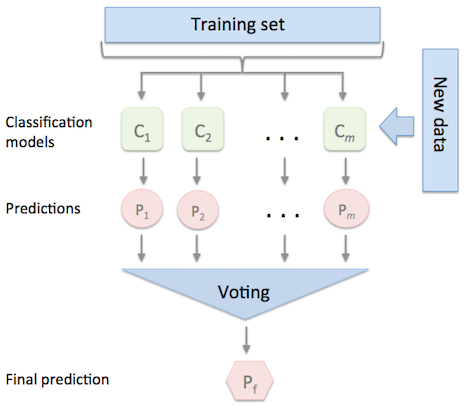
\includegraphics[width=0.7\linewidth]{media/images/majority_voting.png}
    \caption{Explicación gráfica del proceso de entreno y predicción de un \textit{Voting Classifier}. Fuente \cite{Ensemble96:online}.}\ \label{fig:voting-classifiers}
\end{figure}

Por otro lado \textit{Bagging Classifier} entrena el mismo modelo sobre un subconjunto aleatorio del \textit{dataset} y luego agrega los resultados de las predicciones, ya sea haciendo la media o realizando una votación, para obtener una predicción final.\ \cite{sklearne53:online}


Antes de entrenar estos modelos, hemos de decidir qué otros modelos los compondran, por lo tanto, haremos antes un poco de \textit{hyperparameter tuning}, como comentamos en la sección \ref{sec:i1-seleccion}, para tratar de mejorar los modelos base con los que compondremos tanto el \textit{Voting Classifier} como \textit{Bagging Classifier}.

Para hacer \textit{hyperparameter tuning}, seleccionamos primero los modelos que ajustaremos, los cuales son los que mejores resultados han dado del entreno básico, es decir, \textit{Multi-Layer Perceptron, Random Forest, Quadratic Discriminant Analysis y Extra Trees}. De los cuales hemos obtenido los resultados de la \textit{tabla\ \ref{tab:hyperparameter-tuning-results-v2}} donde vemos que tanto \textit{et} como \textit{mlp} han mejorado (aun haciendo \textit{overfitting}), \textit{qda} sigue igual y \textit{rf} ha empeorado. De todas formas, nos sirven los parámetros que hemos encontrado, pues tienen resultados bastante buenos, por lo tanto montaremos tanto el \textit{Voting Classifier} como el \textit{Bagging Classifier} sobre estos.


\begin{table}[!ht]
    \centering
    \resizebox{\textwidth}{!}{\begin{tabular}{|c|ccccccccc|} \hline
        Model name & Train score & Accuracy & Recall & Precision & f1 score & f0.5 score & f2 score & ROC/AUC score & Balanced accuracy \\ \hline
        GS - et & 100 & 95.981 & 93.352 & 98.538 & 95.875 & 97.455 & 94.345 & 95.981 & 95.981 \\
        RS - qda & 91.62 & 91.413 & 82.825 & 100 & 90.606 & 96.018 & 85.772 & 91.413 & 91.413 \\
        GS - qda & 91.62 & 91.413 & 82.825 & 100 & 90.606 & 96.018 & 85.772 & 91.413 & 91.413 \\
        RS - et & 97.778 & 93.487 & 89.474 & 97.289 & 93.218 & 95.619 & 90.935 & 93.487 & 93.487 \\
        RS - mlp & 100 & 94.039 & 91.967 & 95.954 & 93.918 & 95.129 & 92.737 & 94.039 & 94.039 \\
        GS - mlp & 100 & 94.039 & 91.967 & 95.954 & 93.918 & 95.129 & 92.737 & 94.039 & 94.039 \\
        RS - rf & 89.074 & 89.193 & 81.163 & 96.7 & 88.253 & 93.134 & 83.858 & 89.193 & 89.193 \\
        GS - rf & 88.889 & 88.916 & 80.609 & 96.678 & 87.915 & 92.971 & 83.381 & 88.916 & 88.916 \\ \hline
        \end{tabular}}
        \caption{Resultado del \textit{hyperparameter tuning} con el \textit{dataset} balanceado. Fuente propia.}\ \label{tab:hyperparameter-tuning-results-v2}
\end{table}


Al entrenar los \textit{Voting} y \textit{Bagging Classifiers}, obtenemos los resultados de la \textit{tabla\ \ref{tab:voting-bagging-results}}. En general, los \textit{Voting} han obtenido resultados algo mejores que los \textit{Bagging Classifiers}, podría ser por la cantidad de datos sobre los que ha entrenado cada submodelo. De todas formas, en general, obtenemos mejores resultados que utilizando modelo básicos.

\begin{table}[!ht]
    \centering
    \resizebox{\textwidth}{!}{\begin{tabular}{|c|ccccccccc|} \hline
        Model name & Train score & Accuracy & Recall & Precision & f1 score & f0.5 score & f2 score & ROC/AUC score & Balanced accuracy \\ \hline
        Voting Classifier (All - not tuned) & 100 & 95.839 & 92.244 & 99.403 & 95.69 & 97.884 & 93.592 & 95.844 & 95.844 \\
        Bagging Classifier (QDA) & 96.9 & 95.284 & 90.859 & 99.696 & 95.072 & 97.794 & 92.499 & 95.29 & 95.29 \\
        Voting Classifier (QDA and ET) & 97.501 & 95.007 & 90.028 & 100 & 94.752 & 97.833 & 91.86 & 95.014 & 95.014 \\
        Voting Classifier (All) & 98.103 & 94.868 & 90.305 & 99.39 & 94.63 & 97.43 & 91.986 & 94.875 & 94.875 \\
        Voting Classifier (RF and ET and QDA) & 97.362 & 94.73 & 89.474 & 100 & 94.444 & 97.701 & 91.398 & 94.737 & 94.737 \\
        Voting Classifier (MLP and ET) & 100 & 93.481 & 91.136 & 95.64 & 93.333 & 94.704 & 92.002 & 93.485 & 93.485 \\
        Bagging Classifier (MLP - not tuned) & 92.92 & 90.846 & 85.873 & 95.385 & 90.379 & 93.317 & 87.62 & 90.853 & 90.853 \\
        Bagging Classifier (RF) & 92.041 & 87.933 & 82.548 & 92.547 & 87.262 & 90.358 & 84.371 & 87.941 & 87.941 \\
        Bagging Classifier (ET) & 89.82 & 87.656 & 82.825 & 91.718 & 87.045 & 89.79 & 84.463 & 87.663 & 87.663 \\ \hline
        \end{tabular}}
        \caption{Resultados de entrenar los diferentes \textit{Voting} y \textit{Bagging Classifiers} que hemos preparado con los resultados del \textit{hyperparameter tuning}. Fuente propia.}\ \label{tab:voting-bagging-results}
\end{table}